\documentclass[hyperref=colorlinks]{beamer}
\mode<presentation>
\usetheme{iclpt}
\setbeamertemplate{navigation symbols}{}
\setbeamertemplate{headline}{
  \begin{beamercolorbox}[leftskip=.2cm,rightskip=.2cm,topskip=.2cm,ht=1.1cm,dp=0.1cm,wd=\textwidth]{institute in head/foot}
    
\includegraphics[height=1cm]{icl.pdf}
    \hfill
%    \includegraphics[height=1cm]{../Pics/ATLAS-Logo-Square-Blue-RGB.png}
%    
\includegraphics[height=1cm]{../Pics/CMS-Color.pdf}
    
\includegraphics[height=1cm]{TalkPics/t2k_logo_large.png}

%??put t2k logo here
  \end{beamercolorbox}
}
\setbeamertemplate{footline}{
  \begin{beamercolorbox}[ht=.35cm,dp=0.2cm,wd=\textwidth,leftskip=.3cm]{author in head/foot}%
    \begin{minipage}[c]{5cm}%
      \usebeamerfont{author in head/foot}
      \insertshortauthor 
      \insertshorttitle
    \end{minipage}\hfill%
    \hfill
    \insertframenumber{} / \ref{lastframe}
    %\hfill
    \begin{minipage}{6cm}
      \hfill
      %\insertshorttitle
    \end{minipage}
  \end{beamercolorbox}%
}

\definecolor{beamer@icdarkblue}{RGB}{0,51,102}
\definecolor{beamer@icmiddleblue}{RGB}{0,82,150} 
\definecolor{beamer@iclightblue}{RGB}{200,212,232}
\definecolor{beamer@icmiddlered}{RGB}{204,51,0}
\definecolor{beamer@iclightred}{RGB}{232,212,32}

\usepackage{tikz}
\usetikzlibrary{arrows,shapes,backgrounds}
\usepackage{color}
\usepackage{tabularx,colortbl}
\usepackage{graphicx}
\usepackage{pdfpages}
\usepackage{feynmp}
\usepackage{rotating}
\usepackage{moresize}
\usepackage{slashed}
\usepackage{xcolor,colortbl}
\DeclareGraphicsRule{*}{mps}{*}{}
\hypersetup{colorlinks=false}

\title[Xsec Update]{\vspace{-0.2cm} New Xsec Parameterisation Update}
\author[P. Dunne]{Patrick Dunne - Imperial College London}
\titlegraphic{
  \vspace{-0.4cm}
}
\date{}
\begin{document}
\tikzstyle{every picture}+=[remember picture]
\tikzstyle{na} = [baseline=-.5ex]
\begin{fmffile}{t2ktemplatefeyndiags}


  %TITLE PAGE
  %20 mins + 5 questions
  \section{Title}
  \begin{frame}
    \titlepage
  \end{frame}

  \begin{frame}
    \frametitle{Introduction}
    \begin{block}{}
        \scriptsize
        \begin{itemize}
        \item Caveat: Not a NIWG expert
        \item[-] Several figures taken from Kendall, Matt and Patrick S
        \item Will summarise proposed changes for the summer analyses
        \item[-] 2p2h shape, BeRPA, non-dipole axial form factors, Eb
        \item[-] Don't expect any change in tunings but will check matrix when done
        \item Will give progress of implementation and validation
      \end{itemize}
    \end{block}
  \end{frame}
  
  \begin{frame}
    \frametitle{2p2h shape}
    \begin{itemize}
    \item 2p2h split into two components: PDD and non-PDD (+interference)
    \end{itemize}
    \centering
    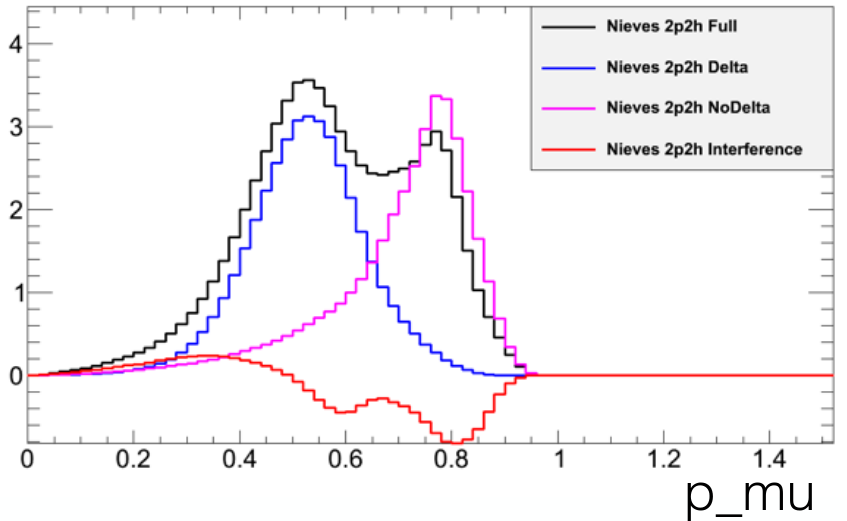
\includegraphics[width=.5\textwidth]{TalkPics/XsecUpdate_070217/pddvsnonpdd.png}
  \end{frame}

  \begin{frame}
    \frametitle{2p2h shape}
    %??Asher's formula and update to take into account variation as a function of energy (was just c flat at 0.5 before not c*Td)
    \centering
    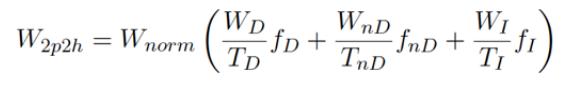
\includegraphics[width=.7\textwidth]{TalkPics/XsecUpdate_070217/2p2hequation.png}
    \begin{itemize}
    \item Mix delta, non-delta and interference parts
    \item[-] W is targeted fraction
    \item[-] T is integrated fraction in nominal
    \item[-] f is fraction in a particular bin
    \item Components add to 1 e.g. $W_{D}+W_{nD}+W_{I}=1$
    \item Tweak method chosen to ensure $W_{D}$ and $W_{nD}$ fractions vary (see backup)
    \end{itemize}
  \end{frame}

  \begin{frame}
    \frametitle{2p2h shape}
    \begin{itemize}
    \item Plus and minus 1 variations move in the direction expected
    \end{itemize}
    \centering
    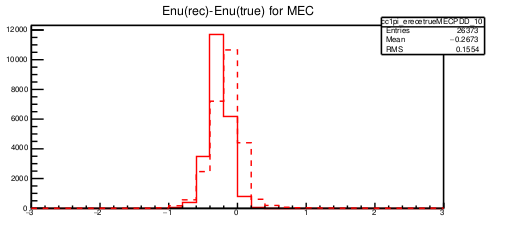
\includegraphics[width=.8\textwidth]{TalkPics/XsecUpdate_070217/2p2hplus1.png}
  \end{frame}

  \begin{frame}
    \frametitle{2p2h shape}
    \begin{itemize}
    \item Plus and minus 1 variations move in the direction expected
    \end{itemize}
    \centering
    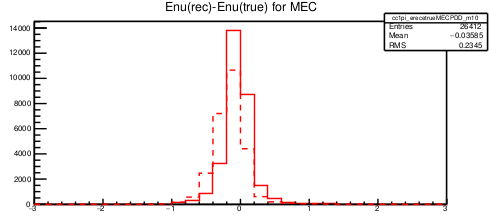
\includegraphics[width=.8\textwidth]{TalkPics/XsecUpdate_070217/2p2hminus1.png}
  \end{frame}

  \begin{frame}
    \frametitle{2p2h shape}
    \begin{itemize}
    \item Problems seen with zero tweak not returning nominal distribution
    \item[-] Believed to be due to dial not being initialised
    \end{itemize}
    \centering
    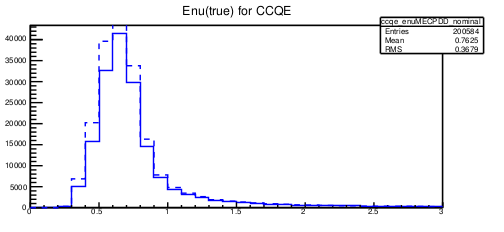
\includegraphics[width=.8\textwidth]{TalkPics/XsecUpdate_070217/2p2hnominalproblem.png}
  \end{frame}

  \begin{frame}
    \frametitle{BeRPA}
    \begin{itemize}
    \item Introduced to allow continuous variation of RPA
    \item Define a functional form and fit to RPA and errors to get nominal and uncertainty: 
      \begin{equation*}
        f(x)=\begin{cases}
        A(1-x)^3 + 3B(1-x)^2 x + 3\alpha(1-x)x^2 + Cx^3, q^{2}<U \\
        1+\left(C-1\right)e^{-D\left(q^{2}-U\right)}, q^{2} \geq U
        \end{cases}
      \end{equation*}
      \item[-] $\alpha$ fixed by continuity
    \item SK Implement as event by event weight in mtuples for nominal
    \item[-] Variations around that nominal done with splines
    \item[-] Have implemented a dial for U, A, B, C, D and Unom, Anom, Bnom, Cnom, Dnom
    \item ND280 use event by event for nominal and variations
    \end{itemize}
  \end{frame}

  \begin{frame}
    \frametitle{BeRPA}
    \begin{itemize}
    \item Varies as expected as each dial is varied
    \item[-] Affected by 2p2h zero tweak not returning nominal issue
    \end{itemize}
    \centering
    \includegraphics<1>[width=.7\textwidth]{TalkPics/XsecUpdate_070217/berpa_a_summary.pdf}
    \includegraphics<2>[width=.7\textwidth]{TalkPics/XsecUpdate_070217/berpa_b_summary.pdf}
    \includegraphics<3>[width=.7\textwidth]{TalkPics/XsecUpdate_070217/berpa_c_summary.pdf}
    \includegraphics<4>[width=.7\textwidth]{TalkPics/XsecUpdate_070217/berpa_d_summary.pdf}
  \end{frame}

  \begin{frame}
    \frametitle{Non-dipole axial form factors}
    \begin{itemize}
    \item Axial form factors previously assumed to be dipole
    \item This gives quite small uncertainties in high $Q^2$ despite not much data
    \item Patrick S has implemented new form factors \textcolor{beamer@icmiddleblue}{\hyperlink{http://www.t2k.org/asg/xsec/meetings/2017/niwg-premeetings-febr2017/axialffupdate}{see here}}
    \item[-] Current plan is to understand with fake data study, but Will be in T2KReWeight for ease of studies
    \end{itemize}
    %Patrick S's stuff as fake data (kendall to send background info) dipole->non-dipole form factor. Dipole has very tight error bands, constrains in region where not so much data but problem for 4pi. Z-expansion and 3 component z-expansion suggested    
    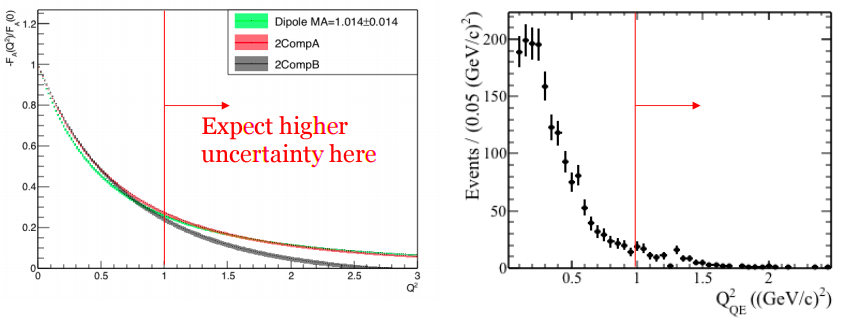
\includegraphics[width=\textwidth]{TalkPics/XsecUpdate_070217/axialffuncertainty.png}
  \end{frame}
  
  \begin{frame}
    \frametitle{$E_{b}$}
    \begin{itemize}
    \item RFG currently used has a certain value of Eb
    \item Previously did Neut vs Nieves fake data study
    \item Bias seen in fixed energy studies
    \item Studies done into using variable Eb dial
    \end{itemize}
    \centering
    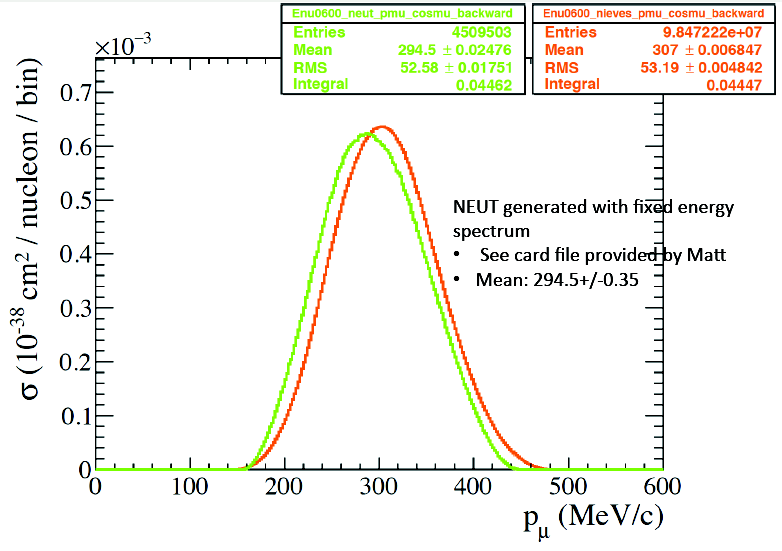
\includegraphics[width=.5\textwidth]{TalkPics/XsecUpdate_070217/ebbiasissue.png}
  \end{frame}

  \begin{frame}
    \frametitle{$E_{b}$ dial studies}
    \begin{columns}
      \column{.5\textwidth}
      \begin{itemize}
      \item Saw issues due to different phase space of RFG models with different Eb
      \item[-] Red where there is no blue
      \item Recoverable because RFG is reweighted from SF which has larger phase space
      \end{itemize}
      \column{.5\textwidth}
      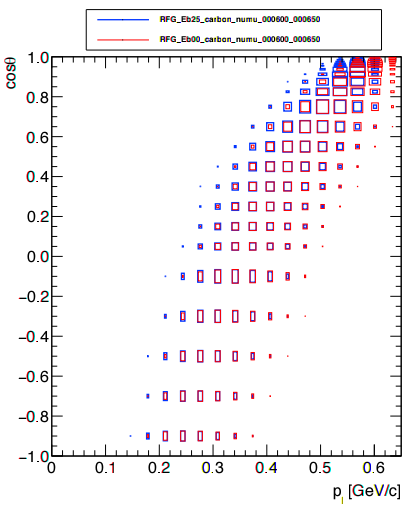
\includegraphics[width=\textwidth]{TalkPics/XsecUpdate_070217/rfgvsrfg.png}
    \end{columns}
  \end{frame}

  \begin{frame}
    \frametitle{$E_{b}$ dial studies}
    \begin{columns}
      \column{.5\textwidth}
      \begin{itemize}
      \item Also problem with RFG phase space where no SF phase space
      \item Red where there is no black
      \item[-] Fix with lower limit on Eb of 14 MeV
        
      \end{itemize}
      \column{.5\textwidth}
      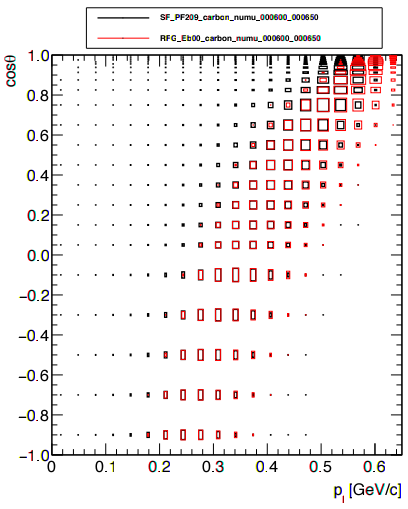
\includegraphics[width=\textwidth]{TalkPics/XsecUpdate_070217/sfvsrfg.png}
    \end{columns}
    %?? Have a plan but it's not a quick fix so will be for after summer analysis. For general background look at Kendall's slides
  \end{frame}

  \begin{frame}
    \frametitle{$E_{b}$ dial studies}
    \begin{itemize}
    \item After fix for both of the above bias still seen
    \item Remaining bias believed to be incompatibility between Eb event by event reweighting and template SF$\rightarrow$RFG reweighting
    \item[-] Idea to fix but will take too long
    \item Should still do Neut vs Nieves fake data
    \item Possibly also fake data vs other Eb values to make sure bias isn't too large
    \end{itemize}
  \end{frame}
  

  \begin{frame}
    \frametitle{Conclusions}
    \label{lastframe}
    \begin{block}{}
      \begin{itemize}
      \item Final proposal to NIWG this afternoon
      \item Main change from old model will be addition of 2p2h shape dial and BeRPA dial and nominal weight
      \item 2p2h nominal issue is being debugged
      \item BeRPA nominal weight replaces RPA weight
      \item Will have fake data studies for Eb, and axial form factors
      \item Other elements same as old parameterisation
      \end{itemize}
    \end{block}
  \end{frame}

  %Backup goes here
  

\begin{frame}
  \centering
  \huge \textcolor{beamer@icmiddleblue}{Backup}
\end{frame}

\begin{frame}
  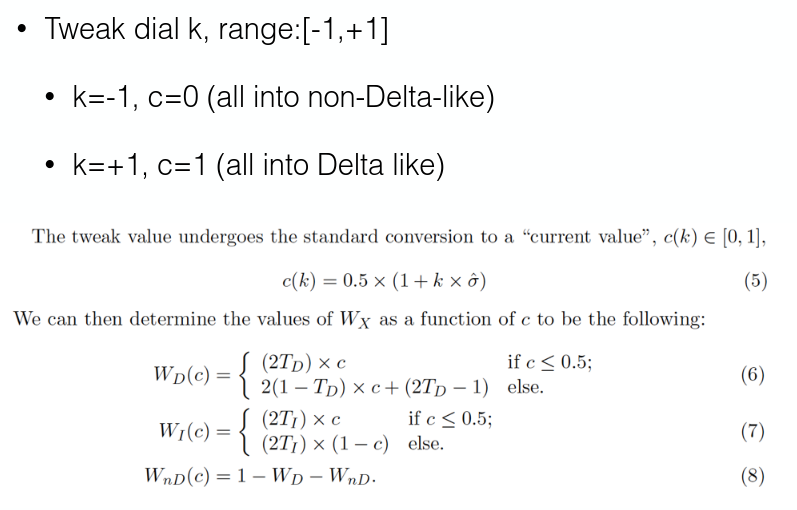
\includegraphics[width=\textwidth]{TalkPics/XsecUpdate_070217/2p2htweakdetails.png}
\end{frame}

\end{fmffile}
\end{document}
